\documentclass[bibliography=totoc, captions=tableheading, titlepage=firstiscover]{scrartcl} %Literatur im Inhaltsverzeichnis, Tabellenüberschrift, erste Seite Titelseite

% Zahlen und Einheiten

%\usepackage[version=4, math-greek=default, text-greek=default]{mhchem}% chemische Formeln
\usepackage{xfrac}% schöne Brüche im Text
\usepackage{scrhack} % Paket float verbessern
\usepackage[aux]{rerunfilecheck} % Warnung, falls nochmal kompiliert werden muss

\usepackage{amsmath} % unverzichtbare Mathe-Befehle
\usepackage{mathtools} % Erweiterungen für amsmath
\usepackage{amssymb} % viele Mathe-Symbole
\usepackage{fontspec} % Fonteinstellungen
% Latin Modern Fonts werden automatisch geladen 
% Alternativ zum Beispiel:
%\setromanfont{Libertinus Serif}
% \setsansfont{Libertinus Sans}
% \setmonofont{Libertinus Mono}

% Wenn man andere Schriftarten gesetzt hat, sollte man das Seiten-Layout neu berechnen lassen
\recalctypearea{}

\usepackage[math-style=ISO, bold-style=ISO, sans-style=italic, nabla=upright, partial=upright, warnings-off={mathtools-colon, mathtools-overbracket}]{unicode-math}

% traditionelle Fonts für Mathematik
\setmathfont{Latin Modern Math}
% Alternativ zum Beispiel:
%\setmathfont{Libertinus Math}

\setmathfont{XITS Math}[range={scr, bfscr}]
\setmathfont{XITS Math}[range={cal, bfcal}, StylisticSet=1]

\usepackage[autostyle]{csquotes} % richtige Anführungszeichen
\usepackage{float} % Standardplatzierung für Floats einstellen
\floatplacement{figure}{htbp}
\floatplacement{table}{htbp}
\usepackage[section, below]{placeins} % Floats innerhalb einer Section halten
\usepackage{pdflscape} % Seite drehen für breite Tabellen: landscape Umgebung
\usepackage[labelfont=bf, font=small, width=0.9\textwidth]{caption} % Captions schöner machen.
\usepackage{subcaption} % subfigure, subtable, subref
\usepackage{graphicx} % Grafiken können eingebunden werde
\usepackage{booktabs} % schöne Tabellen
\usepackage{microtype} % Verbesserungen am Schriftbild
\usepackage[backend=biber]{biblatex} % Literaturverzeichnis
\addbibresource{sample.bib} % Quellendatenbank
%\addbibresource{programme.bib}
\usepackage[german, unicode, pdfusetitle, pdfcreator={}, pdfproducer={}]{hyperref}
\usepackage{bookmark} % erweiterte Bookmarks im PDF
\usepackage[shortcuts]{extdash} % Trennung von Wörtern mit Strichen
\usepackage{url} 
% cover sheet:
\subject{Documentation of the Fachprojekt}
\title{FP7-T4: Deploy Machine Learning Applications on A Swarm} 

\author{Jan Marre\\\href{mailto:jan.marre@tu-dortmund.de}{jan.marre@tu-dortmund.de}\and Sascha Weller\\ \href{mailto:sascha.weller@tu-dortmund.de}{sascha.weller@tu-dortmund.de} \and Ben Raffetseder\\\href{mailto:ben.raffetseder@tu-dortmund.de}{ben.raffetseder@tu-dortmund.de} \and Lukas Schneider\\\href{mailto:lukas2.schneider@tu-dortmund.de}{lukas2.schneider@tu-dortmund.de}}
\publishers{TU Dortmund – Fakultät Informatik}

\date{SoSe21}
% cover sheet Endehttps://www.overleaf.com/project/6130a0989f3465c5d25085a2 


\begin{document} % Protokollanfang 

\maketitle % Generiert Deckblatt

\tableofcontents % Inhaltsverzeichnis
\newpage

\section{Introduction} \label{sec:Intro}

With an increasingly use of drone in different areas such as agriculture, construction and parcel delivery there is also a growing number of use cases for machine learning algorithms. Due to reduced hardware costs and advantages that come with multiple drones working together – swarms of drones where the drones communicate with each other and deploy machine learning algorithms together are going to be used more and more in the coming years. The use of swarms can prevent the unprecedented growth of data collections as well as reducing the complexity of algorithmic solutions needed for solving complex problems. \\
However, before implementing complex machine learning algorithms on swarms there are several challenges that must be tackled as for example parallelisation of algorithms, statistical heterogeneity or the limited performance of the single drones. \\
In order to build a solid foundation for the implementation of other machine learning algorithms, the Fachprojekt “Digital Design for Machine Learning” focuses on the implementation of a machine-learning-framework. This framework will provide the basic functionality for the deployment of more complex algorithms on STM32 hardware (and other hardware) that can be used for well scaling drone swarms.
 

\section{Motivation} \label{sec:Mot}
Alongside the distribution of machine learning algorithms on distributed platforms come several challenges that must be considered.
\begin{enumerate}
    \item The ML-Algorithms need to have a high degree of parallelism, so we can make use of the distributed computational power.
    \item The performance of the hardware and the workload on each drone needs to be considered.
    \item Communication between the drones is highly resource expensive and therefore needs to be reduces to an absolute minimum.
    \item Data collected from different drones might show statistical heterogeneity if the collection is not well implemented.
\end{enumerate}
Problems that normally come with distributed machine learning are privacy and system heterogeneity, but because we assume using the same hardware for all the drones, we can ignore problems that come with system heterogeneity. Privacy concerns are negligible as well because we are going to reduce the communication to the sending results of aggregation and updated weights only and therefore no sensitive data can be derived from this data. \\
For testing the framework, we will implement random forest as machine learning algorithm in order to classify the data received. 



\section{Theory}
This chapter gives a short overview of the theory behind distributed machine learning which was used for the swarm design. Chapter 3.1 therefore gives a short introduction to the different design aspects one has to take into consideration and is mainly based on \cite{DBLP} and \cite{article}. In chapter 3.2 the theory behind Decision Trees and Random Forests as they are later will be used for the drone swarm.  

\subsection{An Overview on distributed Machine Learning}

When designing an distributed Machine Learning architecture different aspects have to be taken into account. Mainly decisions on the use of the machine learning algorithm, the parallelism of the model and the topology while taking into account the used hardware and the data \cite{DBLP}. \\

The machine learning algorithms can be classified by their feedback(e.g. supervised or unsupervised learning), purpose and method. With the purpose of an ML algorithm the task it is used for is described, like classification, clustering or regression. The method is the selected way the algorithm improves according to the imput data. Popular methods include Stochastic Gradient Descent algorithms (e.g. Support Vector Machines, Artificial Neural Networks), Evolutionary Algorithms or rule-based algorithms(e.g. Decision Trees).  \\

\begin{figure}
	\centering
	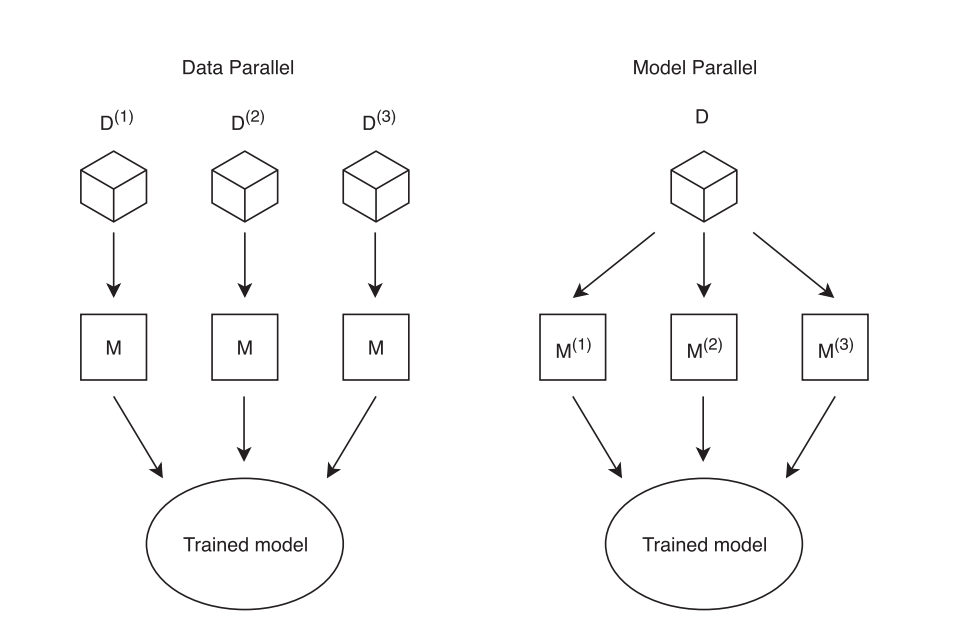
\includegraphics[width=0.5\textwidth]{scalingout.PNG}
	\caption{Difference between Data Parallel and Model Parallel Architectures[A].}
	\label{fig:Parallel}
\end{figure}

When looking into how to distribute the machine learning, a decision has to be made how the parallelism is achieved. The most common used methods are Data Parallel and Model Parallel (Figure\ref{fig:Parallel}). With Data Parallel the training data is partitioned into different sets and then applied to train different instances of the same model. The Model Parallel approach partitions the model itself which is then trained with copies of the same data set. To combine these distributed parts some applications need ensemble methods to aggregate the different results the separate nodes gibe. Some ensemble method include Bucketing where select the model with the best performance is selected, Stacking where the outputs of other models are used as inputs for another model or Random Forests which are described in chapter 3.2. \\  
\begin{figure}
	\centering
	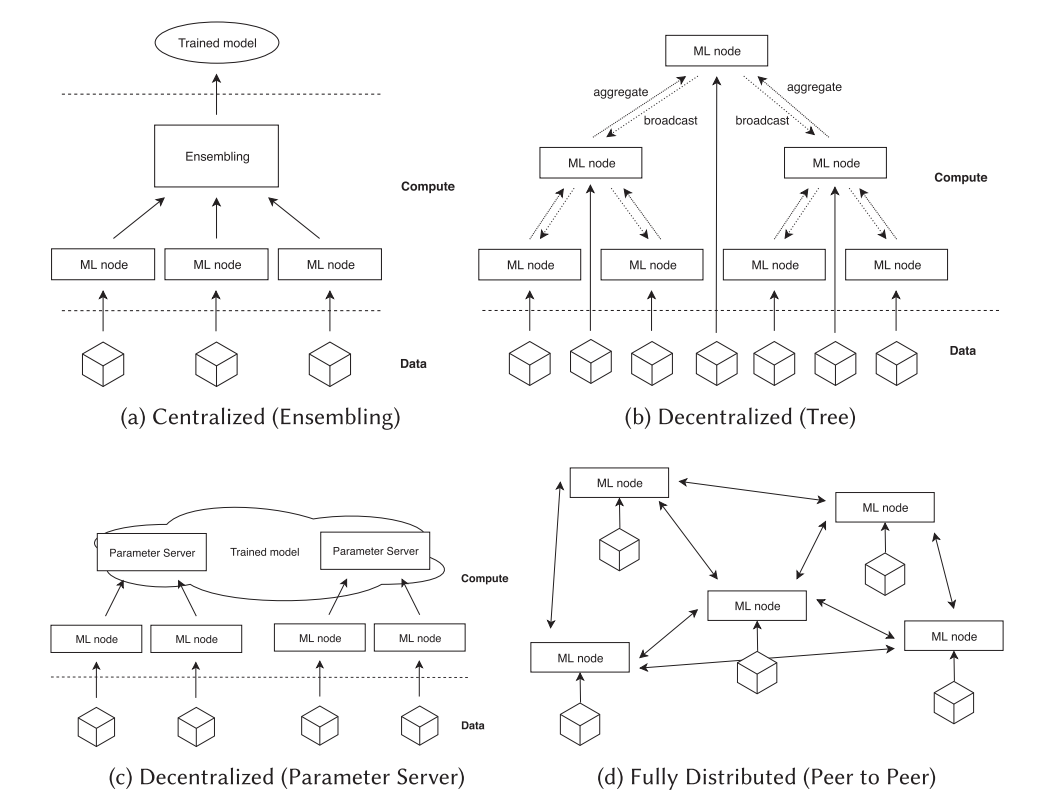
\includegraphics[width=0.5\textwidth]{topologies.PNG}
	\caption{Different possible topologies for distributed machine learning[A].}
	\label{fig:Topo}
\end{figure}


To organize the different nodes within the model, a choice has to be made in what topology the system should be arranged. In Figure 2 some commonly used topologies are shown.  The centralized system connects all nodes through one central server who does the aggregation. In a decentralized system either a tree structure is used to stack different models and allow intermediate aggregation or a Parameter server which connects different parts of a partitioned model. The fully distributed systems implement a peer-to-peer network of all nodes with no hierarchy. 



\subsection{Decision Trees \& Random Forests}

\subsubsection*{Decision Trees}
Decision Trees are a machine learning model which can be used for classification tasks. Therefore when learning the structure  of a decision tree we expect data of the form $D=(X_1,X_2,...,X_n,Y)$ where $Y$ is the variable we want to classify on. The structure of a decision tree consists of decision nodes and classifier nodes as leaves. Each decision node is associated with a variable $X_k$ and has edges to its multiple children. These edges are labeled with a possible value $x_k \in X_k$ so that all outgoing edges of a decision node cover the whole definition space of $X_k$. The classifier nodes at the leaves then represent a fixed value $y \in Y$. \\
For classification of some input data $(x_1,x_2,...,x_n)$ it starts at the root of the tree and follow all the edges down the tree where the value of the decision node matches the one of the edge until it reaches a leave node and returns the found classification $y$ \cite{mitchell1997machine}.

\subsubsection*{ID3}
ID3 is a commonly used, greedy Algorithm which builds a decision tree from training data. As a metric to decide  which variable it chooses for the next decision node the Information Gain is used. This metric uses the Entropy of a set $D$:
\begin{equation*}
    E(D)=\sum_{i=1}^{c} -p_i \log p_i
\end{equation*}

where $p_i$ is the proportion of $X_k$ which belongs to one class $y \in Y$. Therefore the Entropy describes the impurity of a set of training data. With the Information gain we then want to measure how much the selection of a variable $X_k$ for a decision node reduces the impurity within the remaining set:
\begin{equation*}
    I(D,X_k)= E(D) - \sum_{t \in T} P(t) H(t)
\end{equation*}
where $T$ are the subsets created by splitting $D$ on the variable $X_k$. \\
The algorithm then selects iterative the variable with the highest information gain starting at the root until all remaining data belongs to one classification, so a leaf is created \cite{mitchell1997machine}.   
Although the algorithm has some drawbacks, like it not being able to catch dependencies between variables or overfitting to the training data \cite{5991826}, its simplicity makes it very suitable for the limited hardware used in this project.
 

\subsubsection*{Random Forests}
To counteract the limitations a single decision tree has, a Random Forest consisting of several decision trees can be used. For achieving this, the training data is randomly sampled (with replacement) $B$-times into sets $D_B=(X_b,Y_b)$ which are afterwards used to train $B$ different decision trees. \\

The prediction is then done separately on each tree from which we gain $B$ classifications. For a final result the model then takes the mode or mean over all prior results. 


\section{A Machine Learning Approach for a Swarm}

\subsection{The Swarm Design}

The first issue for the swarm design is to choose a suitable topology. One possibility is a decentralised circle or mesh topology, the other option is a star topology with a central node. The second issue is how to create a link between all nodes of the swarm. \\


For our swarm we decided to use the star topology with a Bluetooth link between the central node and the drones. This allows us to use the host-client pattern for communication, so we don’t need to deal with the problems of a decentralised topology and fits with the need of a central node for our approach of distributed machine learning.  \\

Each drone runs two tasks, one is the collection and processing of data the other one is the communication with the host. In our case the data collection is simulated and processed by in random forest instance. After that the drone waits for the incoming link from the host. \\

To establish a link the host can search for a drone by his Bluetooth name or connects directly by the known Bluetooth address. According too the host-client pattern, the host controls the communication with the drones by sending them a message when they should sent their collected am processed data. Ones the host has all data from the drones he need for the machine learning application he processed them and sent his results back to all drones.

\subsection{The Bluetooth Communication}

Ones the host established the link to the drones he can send and receive data from each drone. To collect the data, we need for the machine learning algorithm the host cycle the list with all drones and collects the data from each. \\
For that the host send a communication start massage to the drone, the answer of the drone is the data for the aggregation. The communication sequences ended with the end of this data massage. The established link supplies an input and an output stream. To simplify the usage of the steam we designed a structure for our massages. A massage is structured like the following pattern:
\begin{center}
    \#<length of the payload>|<payload>
\end{center}
With this pattern, characterized by his control characters, we know when a message starts and how long it is.



\section{Implementation}

\subsection{Platforms}
As a platform for the host, we used desktop computer, because of some developing issues. The majority of Bluetooth modules where the integrated modules in the notebooks. We use Java 10 SDK and IntelliJ IDEA as main Java developing software on a 64-bit Windows 10. \\

As a platform for testing the implementation we used the STM32F407 Discovery board \cite{STM32}. It comes with a 32-bit Arm based, single core processor, gets powered by an external power supply of 3 or 5 Volts and is compatible to a variety of different sensors such as temperature, video and audio sensors. Already onboard are an accelerometer, LEDs that we used for debugging (read more at chapter Debugging) and full support for the STM32CubeIDE that is developed by STMicroelectronics as well. 
For the communication we attached a Bluetooth module via a UART Interface to the STM32F407 Discovery board. We choose the HC-05 Bluetooth-Board because it’s very common and well documented. 

\subsection{Software for drone Implementation}
\subsubsection*{IDE}
As mentioned, the board is we used is compatible with the STM32CubeIDE, that we used for implementing the framework as well as the machine learning algorithm. The IDE is based on Eclipse and supports all the add-ons that come with Eclipse. 
The STM32CubeIDE comes with a lot of helpful features such as:
\begin{itemize}
    \item The built in STM32CubeMX that is used for configuring the Pinout, clock of the processor and peripheral hardware.
    \item A code generator that makes the definition and addressing of the different Pins easier. 
    \item Advanced debug features like CPU fault analysis, register views and real-time tracing.
\end{itemize}
For this project we used the 64-bit version for Windows 10 and used the STM32CubeProgrammer in addition for erasing the memory before debugging. 

\subsubsection*{Debugging}
There are different ways for debugging the STM32 boards:
\begin{itemize}
    \item Using the serial cable that we also use to power the STM32F407
    \item Using the special STLink Debugging cable
    \item Using the built-in LEDs 
    \item Reading values directly out of the memory 
\end{itemize}
Unfortunately, we could not get the console input and output to run, therefore we used the built-in LEDs in order to debug our code part by part. The implementation for using the LEDs is quite simple as the right declaration and initialisation is already done by the built-in code generator. We simply used the pre-defined method HAL\_GPIO\_TogglePin() in order to turn on a LED.

\subsubsection*{Programming Languages}
As programming language for the drone, we used C++ because its performance advantages and our previous knowledge. There is also the possibility of using C as well as deploying TensorFlow and, hence using python. However, when using TensorFlow we could not have made use of the features that come alongside the IDE but would have access to a lot of useful libraries for more complex machine learning algorithms. \\
The host runs on a laptop, so we don’t have any restrictions for language by performance and hardware. Our first tests with C and Python failed by a bunch of issues. In Python we had problems with the library PyBluez and in C we aren´t able to use the Bluetooth module of the laptop. So we ended by using Java.

\subsubsection*{Implementing the drone framework and random forest}
When generating a new project within the STM32CubeIDE it auto-generates the main file consisting of the main method and the initialisation of the pins used. \\
In addition to the main class we created another class called decisiontree.cpp that contains the implementation of the Table, Node and DecisionTree objects. The DecisionTree object is later used to build up a decision tree on each drone. When building the tree the drone uses an implementation of the ID3 algorithm (see Chapter 3.2)\cite{BowTree}.\\
The main method basically consists of two main parts, the Initialisation and the while loop. \\
Within the initialisation part we set up empty tables that are then used to learn and save the results. Therefore, we simply initialize the table objects table, obstable (observation table) and restable (result table). Furthermore, a Boolean variable called host is declared and set. This variable determines whether a drone is only there for building a decision tree and later sending it, or if the drone is the host drone/central drone that is responsible for aggregating all the results gathered from the other drones. \\
When entering the while loop, first the role of the drone is checked. If the drone does not need to do the aggregation, it simply builds the decision tree by calling the corresponding method and afterwards sends the leafs of the tree that was generated. \\
If on the other hand the drone needs to do the aggregation, it first of all receives all the results generated by the other drones and then builds the modus (in case of random forest with modus) of all the results. The result can then be sent back to the drones which will give future projects the possibility to send back updated weights when using for example federated machine learning \cite{DBLP:journals/corr/abs-1908-07873}.
The while loop runs indefinite and repeats the same steps again for new data provided by the sensors. 

\subsection{Implementation of the host}
The implementation of the host mostly can be divided in three parts the main class, the client and communication section and the machine learning part. \\
The host is the main class which handles the dones, each as a separate client object, collect their data and passes them to the aggregation function of the machine learning algorithm. In the initiation phase the host creates for each drone a separate object by calling the client constructor with the Bluetooth address of the drone. If the Adress is unknown its possible to use the scanner to search by the device name. Ones the initiation is done the main loop start. In the main loop the host connects to all drones after another and collects they’re processed data for the aggregation. After the aggregation the new weights for the random forest algorithm on the drones were sent to them. \\
To the client and communication section belong two classes, the first is the client class. The client class contains the constructures for creating a client object by his Bluetooth adress. The class also contains the methods to init, establish and close the Bluetooth link, as well as the methods to send to - and read from the drone.
The BluetoothScanner class contains the methods to search for a drone by the Bluetooth name. \\
The third section is machine learning section. In the ML-Section the collected data is processed.  


\section{Experiments}
This chapter consists of the experimental evaluation of the distributed machine learning in the Drone Network described in the previous chapters. In the first part it is explained how the different data sets were pre-processed to overcome the hardware limitations. Afterwards a short overview of the different experiments and the used metrics for evaluation is given. Then the results are presented and later discussed in chapter 7.

\subsection*{Data Preparation}
Due to hardware limitations, which would not allocate the storage for the String datatype properly,the mostly categorical data had to be pre-processed. Therefore a python script was developed which mapped all String values within one data set to predefined Integer values which then worked on the board. Afterwards it build a String version of the set so it could be copied into the main-method of the drone software as the data had to be hard-coded and could not be read from a file. 
\subsection*{Overview}
The experiments were executed using three different data sets on a Swarm of size $|N| = 2$. The data sets used were \textit{balance-scale}, \textit{breast-cancer} and \textit{car} from \cite{Dua:2019}. For the first set weights and positions of objects on a scale is given and the model should classify to what side the scale tilts. In the second set data of different patients with breast cancer is given and the classification is about whether it recurred. The data given in the last set consists of multiple attributes of a car and the model should classify if it is accountable. \\
All three sets were prepared as described before and then randomly split into three sets $D_1,D_2,D_t$ which all three had the size $D_n = 36$ due to storage limitations on the board. $D_1$ and $D_2$ were used as data-parallel input for training the models on the two drones so that both could afterwards classify $D_t$ and send it to the central server. \\
The final classification of the server was then evaluated using different metrics. First a confusion matrix was build which plots the real classes of $D_t$ with the predicted classes normalised over the number of real classes in the data set. Then three different scores were measured:

\begin{itemize}
            \item $Precision(x) = \frac{\#correctpredictions(x)}{\#allpredicitions(x)}$
            \vskip .1in
            \item $Recall(x) = \frac{\#correctpredictions(x)}{\#realclasses(x)}$
            \vskip .1in
            \item $F1(x) = 2 * \frac{Precision(x)*Recall(x)}{Precision(x)+Recall(x)}$
\end{itemize}

\newpage
\begin{center}
\subsection*{Results}
\begin{table}[]
\centering
\begin{tabular}{c|ccc ||ccc}
\begin{tabular}[c]{@{}c@{}} real class\\ /predicted class\end{tabular} & Left & Balanced & Right & precision & recall & F1 \\ \hline
Left     & 0,69 & 1 & 0,35 & 0,58 & 0,69 & 0,63\\
Balanced & 0,25 & 0 & 0,25 & 0    & 0    & / \\
Right    & 0,06 & 0 & 0,40 & 0,89 & 0,4  & 0,55 \\ \hline
Avg      & & & & 0,49 & 0,36 & 0,59
\end{tabular}
\caption{Results for \textit{balance-scale} dataset}
\end{table}


\begin{table}[]
\centering
\begin{tabular}{c|cc ||ccc}
\begin{tabular}[c]{@{}c@{}} real classification\\ /predicted class\end{tabular} & No   & Yes  & precision & recall & F1\\ \hline
No                                                                      & 0,84 & 0,75 & 0,8  & 0,84 & 0,82\\
Yes                                                                     & 0,16 & 0,25 & 0,29 & 0,25 & 0,27 \\ \hline
Avg & & & 0,55 & 0,55 & 0,55
\end{tabular}
\caption{Results for \textit{breast-cancer} dataset}
\end{table}


\begin{table}[]
\centering
\begin{tabular}{c|cccc ||ccc}
\begin{tabular}[c]{@{}c@{}} real classification\\ /predicted class\end{tabular} & Unaccaptable & Acceptable & Good & Very Good & precision & recall & F1 \\ \hline
Unaccaptable & 0,55 & 0    & 0 & 0 & 1    & 0,55 & 0,71   \\
Acceptable   & 0,34 & 0,67 & 0 & 0,20 & 0,15 & 0,67 & 0,25\\
Good         & 0,03 & 0,33 & 0 & 0  & 0    & /    & /   \\
Very Good    & 0,07 & 0    & 0 & 0,80 & 0,67 & 0,80 & 0,73 \\ \hline
Avg         & & & & & 0.61 & 0,67 & 0,56
\end{tabular}
\caption{Results for \textit{car} dataset}
\end{table}
\end{center}

\newpage

\section{Discussion}
\subsection*{Experiments}
As it can be seen in the results (Table 1-3) the trained model did have a high amount of overfitting to the train data set and therefore did a lot of miss-classifications. For example the \textit{Yes}-classification in the \textit{breast-cancer} set was mostly predicted as \textit{Yes} and the \textit{Acceptable}-class in \textit{car} was predicted to often as well as the \textit{Balanced}-class in \textit{balance-scale}. These lacking results can be mostly explained by the limitations of used hardware. The very small size of the training data sets on each board is the main problem which caused the overfitting. This could then not be overcome by the Random Forest of the multiple drones due to the small swarm size where calculating the mode is not very representative. \\
Although the experimental results had a limited outcome, the main goal of the Fachprojekt was still achieved, which was to show that these machine learning applications can be executed on the limited hardware. For more detailed performance evaluation of the ID3 algorithm and Random Forests themselves refer to \cite{5991826} and \cite{RODRIGUEZGALIANO201293}. 

\subsection*{Limitations of our approach}
During the implementation and experiment phase we have to deal with some limitations of our approach.
On the one hand are the limitations coursed by design and used technologies like range limitations or memory issues.
On the other hand are the limitations coursed by our implementation.

Since we use an MCU for our application the memory is very limited.
This constrain is important because we used hard coded data for our application, so we can us only a data set with 36 entries in our experiments.
Due to a memory allocation failure of the STM we need to encode our data as integer and not as planned as strings.
The expansion of the swarm is limited by the used technology, in our case the range of Bluetooth.\\
Our implementation generate also some issues, for example we didn't implement error handling.  

\subsection*{Possible upgrades for the future}
Due the known limitations and some inspirations from other technologies are some upgrades for the future given or necessary for future use and development.
One of this necessary upgrades is multi threading, so the ML-Algorithm and the Communication run in parallel.
For the ML-Algorithm its maybe use full to implement some kind of buffer, so the Drone can classify more the one object before sending the classification to the host.
And a possible upgrade for the host is a way to broadcast new weights for the ML-Application to all drones at ones.

\newpage

\printbibliography

\end{document}